\documentclass{article}
\usepackage[T1]{fontenc}
\usepackage{lmodern}
\usepackage{graphicx}
\usepackage{amsmath,amssymb}
\usepackage[a4paper,margin=2cm]{geometry}
\usepackage[absolute,overlay]{textpos}
\setlength{\TPHorizModule}{1mm}
\setlength{\TPVertModule}{1mm}
\usepackage[indonesian]{babel}
\usepackage{hyperref}
\setlength{\emergencystretch}{2em}
% unit: Halaman 23

\begin{document}

% === Halaman 23 (python/native) ===

Pejabat eksekutif operasi khusus dari Inggris 

memperlihatkan syal yang bertuliskan kunci 

OTP selama PD II

• OTP pernah digunakan oleh mata-mata (spy) selama Perang Dunia II

Sumber: John H Reif, History of Computing, 

Duke University


23

% deskripsi: gambar native xref 108
\noindent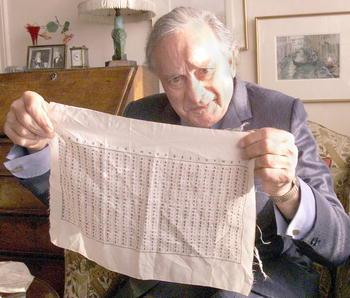
\includegraphics[width=0.85\textwidth]{../../images/python/page_023_img_01.jpeg}

\end{document}
